\documentclass[10pt,a4paper]{article}
\usepackage[margin=18mm]{geometry}
\usepackage[T1]{fontenc}
\usepackage{lmodern}
\usepackage[utf8]{inputenc}
\usepackage{amsmath,amssymb}
\usepackage{booktabs}
\usepackage{graphicx}
\usepackage{caption}
\usepackage{hyperref}
\usepackage{url}
\usepackage{float}
\usepackage{enumitem}
\hypersetup{colorlinks=true,linkcolor=blue,citecolor=blue,urlcolor=blue}
\graphicspath{{figures/}}
\setlength{\parskip}{0.3em}
\setlength{\parindent}{0pt}
\setlength{\textfloatsep}{8pt plus 2pt minus 2pt}
\setlength{\intextsep}{8pt plus 2pt minus 2pt}
\setlength{\floatsep}{8pt plus 2pt minus 2pt}
\captionsetup{font=small,labelfont=bf}

\title{\textbf{From RTL to GDSII: A Reproducible Open-Source\\
Workflow Study of GPU-Style ASIC Kernels}}
\author{Pankaj Thakur\\Roll No. 24dec019
  \and Shubham Pathania\\Roll No. 24dec026
  \and Rahul Sharma\\Roll No. 24dec021}
\date{3 November 2026}

\begin{document}
\maketitle

\begin{abstract}
This paper follows two RTL kernels through an open-source ASIC design flow:
a fixed-point triangle rasterizer and a 4-by-4 signed INT8 matrix tile. The
three rasterizer variants were simulated and taken through matched
OpenLane/Sky130A runs, from synthesis to GDSII. A testbench also drives the
matrix tile through a 90-by-90 multiplication in simulation; the saved
matrix GDSII is for the 4-by-4 tile, not a 90-by-90 array.

Each rasterizer was checked against a bit-exact reference for 136 triangles
(34,816 pixel comparisons per implementation; 104,448 across all three).
The matrix benchmark composes the 4-by-4 tile to compute 90-by-90 signed
INT8 inputs with signed 32-bit accumulation, checks all 8,100 outputs, and
reports deterministic RTL cycles. Its tiled driver pads to 92 and submits
12,167 tile jobs. These are simulation results, not silicon throughput. For
the reference and small triangles, clipping reduces scan cycles from 256 to
121 and 4, respectively, while the flow critical-path metric rises from
9.57 ns for direct evaluation to 14.07 ns. The full-frame incremental
variant uses 9.8\% more synthesis area than the direct design without
reducing scan cycles. In the 135 nondegenerate cases in the deterministic
correctness corpus, clipping reduces the mean scan count from 256 to
69.97 cycles and the median from 256 to 49. The corpus includes many
off-screen triangles, so those statistics should not be read as a
production-scene speedup.

All three rasterizers pass the same bit-exact reference suite and have saved
RTL-to-GDS runs. Clipping shortens scans for sparse triangles but increases
physical cost; the direct design has the smallest mapped area and shortest
reported critical path. Multi-corner reports show negative setup slack for
all three designs. The saved OpenLane power results are typical-corner
vectorless estimates, not workload power or energy measurements.
\end{abstract}

\textbf{Keywords:} RTL, triangle rasterization, INT8 matrix multiplication,
Sky130, OpenLane, GPU architecture, ASIC design-space exploration, reproducibility

\section{Study question and scope}

The main question is how edge evaluation and traversal affect correctness,
scan latency, mapped area, and routed timing under one bit-exact coverage
contract. The matrix workload is a separate test of the existing tiled INT8
datapath.

The two kernels perform different functions and use different interfaces,
so their area and timing are reported separately. The 90-by-90 matrix case
is testbench-orchestrated using the existing 4-by-4 RTL tile; it is not a
90-by-90 physical array.

Pineda's edge-function formulation provides the mathematical basis for the
rasterizer \cite{Pineda1988}. Owens et al. survey the broader use of GPUs for
data-parallel computation \cite{OwensGPU2007}; this project implements small
RTL kernels, not a commercial GPU architecture. The study compares exact
edge recurrence and conservative bounding-box traversal under one verified
coverage contract. It does not propose a new rasterization algorithm. The
4-by-4 MAC tile is a separate integer-compute example, not a proxy for
modern tensor-core designs. A fuller literature review is needed before
making a novelty claim. Neither block includes a programmable graphics
pipeline, shared memory, shaders, texture or depth processing, or display
output. The project overview is in
\href{../README.md}{the GPU project README}; the block description is in
\href{../../gpu_triangle/README.md}{the rasterizer README}.

\section{Project structure and implementation}

The source tree separates the kernels, tests, physical runs, and report
artifacts. Table~\ref{tab:project-structure} lists the main paths relative
to \texttt{designs/}.
\begin{table}[!htbp]
\centering
\small
\begin{tabular}{p{0.29\linewidth}p{0.62\linewidth}}
\toprule
Project path & Contents and role\\
\midrule
\texttt{gpu\_triangle/src/} & Direct, incremental, and clipped-incremental
rasterizer RTL implementations (D, I, IB).\\
\texttt{gpu\_triangle/sim/} & Shared correctness, cycle-benchmark, UI, and
waveform testbenches; the reference test checks all framebuffer bits
against an integer oracle.\\
\path{gpu_triangle_incremental/} and
\path{gpu_triangle_incremental_bbox/} & Matched OpenLane configs and
saved RTL-to-GDS runs for I and IB; the direct baseline run is under
\texttt{gpu\_triangle/}.\\
\texttt{gpu4x4/src/}, \texttt{gpu4x4/sim/} & The 4-by-4 INT8 MAC RTL,
tile tests, the 90-by-90 workload, and its saved physical run.\\
\texttt{gpu4x4/research\_report/} & This LaTeX report, references,
reproduction scripts, source logs, machine-readable summaries, and rendered
layout/waveform figures.\\
\path{gpu_16bit/} & Separate OpenLane attempt. It is excluded: the saved run
failed lint because its configured \texttt{src/*.v} files are absent.\\
\bottomrule
\end{tabular}
\caption{Project directories and their roles.}
\label{tab:project-structure}
\end{table}

Icarus Verilog runs the shared rasterizer tests and the matrix benchmarks.
GTKWave exports an RTL trace. OpenLane synthesizes and routes the rasterizer
variants, and KLayout renders their saved GDS files. The report is built
with \texttt{pdflatex} and BibTeX. The ngspice deck checks a Sky130
standard-cell inverter; it does not simulate either accelerator. The RTL
kernels have not been captured as Xschem transistor-level schematics.

\section{Open-source RTL-to-GDSII workflow}

This paper documents one pinned open-source flow, not a comparison of EDA
tools. The rasterizer variants are direct (D), full-frame incremental (I),
and incremental with bounding-box clipping (IB). OpenLane coordinates
Yosys synthesis and OpenROAD physical implementation
\cite{OpenLaneDocs,OpenROADDocs}. The mapped library is
SkyWater's \texttt{sky130\_fd\_sc\_hd} standard-cell library
\cite{Sky130Docs}. The runs use OpenLane v1.0.2, Yosys 0.30+48, and
OpenSTA 2.4.0. The run manifest records the OpenLane and Sky130A PDK
commits; the flow logs record the OpenROAD build. Configuration files set a
20 ns clock target and 35\% core utilization for the matched rasterizer
runs.

\begin{table}[!htbp]
\centering
\small
\begin{tabular}{p{0.20\linewidth}p{0.24\linewidth}p{0.46\linewidth}}
\toprule
Stage & Tool or input & Evidence retained for this project\\
\midrule
RTL and constraints & Verilog sources, OpenLane configuration & Three
rasterizer implementations; clock and core-utilization settings; source and
configuration hashes in \texttt{data/physical\_runs.csv}.\\
Functional checks & Icarus Verilog & 136-triangle oracle regression for
each rasterizer, four fixed cycle benchmarks, matrix-tile tests, and the
90-by-90 testbench result.\\
Lint and synthesis & Verilator and Yosys & OpenLane lint log, mapped
standard-cell netlist, synthesis statistics, and cell-area results.\\
Floorplan and implementation & OpenROAD & Floorplan, power grid, placement,
clock-tree synthesis, global and detailed routing, and intermediate DEF
files.\\
Extraction and analysis & OpenROAD RCX and OpenSTA & Extracted parasitics,
setup/hold timing, multi-corner reports, physical-design checks, and
typical-corner vectorless power estimates.\\
Layout output & OpenLane GDS stream-out; KLayout & Final GDSII files for D,
I, IB, and the separate 4-by-4 matrix tile; rendered figures in
\texttt{research\_report/figures/}.\\
Simulation inspection & GTKWave & VCD-based view of one rasterizer run.
This trace illustrates RTL behavior; it is not cell-level switching
activity for power analysis.\\
\bottomrule
\end{tabular}
\caption{Stages of the RTL-to-GDSII workflow exercised in this project and
the evidence retained at each stage.}
\label{tab:workflow}
\end{table}

The D, I, and IB runs use the same clock target, utilization target, PDK
revision, and standard-cell library. The manifest records source and
configuration hashes for each run. All three produced GDSII, DEF, parasitic
data, and reports. The reports show zero TritonRoute and Magic DRC
violations, but include antenna and fanout warnings. Separate min/nom/max
timing reports show negative setup WNS. The project has no fabricated
silicon, and these runs do not establish all-corner timing closure.

The 4-by-4 matrix tile has its own saved OpenLane run and layout. The
90-by-90 multiplication is a simulation workload driven by the testbench;
it was not synthesized as a 90-by-90 block. Likewise, the GTKWave VCD is
generated from RTL simulation and was not annotated onto the mapped
netlists. OpenSTA's power results are therefore vectorless estimates, not
activity-based power measurements. The reproduction script reruns the RTL
tests and rebuilds the report from retained physical-flow results; it does
not rerun OpenLane.

\subsection{Matrix tile physical run}

The separate matrix-tile run completed and produced GDSII. Its metrics are
shown below for context; they are not part of the D/I/IB comparison because
the matrix tile implements a different workload. The typical-corner setup
slack is positive, while the separate min/nom/max MCA reports have negative
WNS.

\begin{table}[!htbp]
\centering
\small
\begin{tabular}{p{0.56\linewidth}p{0.36\linewidth}}
\toprule
Metric & 4-by-4 matrix tile\\
\midrule
OpenLane run & \url{RUN_2026.11.02_21.13.38}\\
Mapped synthesis cells & 11,858\\
Final DEF die area (\(\mathrm{mm}^2\)) & 0.35658\\
Flow critical-path metric (\(\mathrm{ns}\)) & 2.97\\
Final \texttt{31-rcx} setup slack (\(\mathrm{ns}\)) & 8.78\\
MCA setup WNS, min/nom/max (\(\mathrm{ns}\)) & \(-0.07/-0.38/-0.68\)\\
TritonRoute/Magic DRC violations & \(0/0\)\\
Max-fanout violations & 37\\
Antenna pin/net violations & \(25/22\)\\
Typical-corner vectorless power (mW) & 41.0\\
\bottomrule
\end{tabular}
\caption{Saved OpenLane results for the 4-by-4 matrix tile. The
single-corner slack and multi-corner WNS come from separate reports. Power
is vectorless and has no workload activity annotation.}
\label{tab:matrix-physical}
\end{table}

\texttt{gpu\_16bit/} is a separate, incomplete flow attempt. Its saved run
stopped at Verilator lint because the configured \texttt{src/*.v} files are
missing. It has no RTL or GDSII result and is excluded from this study.

\section{Implemented hardware}

\subsection{Fixed-point triangle coverage}

\paragraph{Mathematical and architectural lineage.}
The signed edge-function model follows Pineda's parallel polygon
rasterization formulation \cite{Pineda1988}. The per-pixel recurrence is
derived exactly from its determinant; it is not a new coverage rule.
Pixel-center sampling and inclusive edges are this project's contract.
Documented graphics API rules, such as Direct3D's, illustrate why edge
ownership must be specified \cite{MicrosoftRasterization}. The high-level
architecture motivation is the separation of graphics-pipeline and
data-parallel-compute workloads surveyed by Owens et al.
\cite{OwensGPU2007}. No proprietary vendor pipeline or datapath is claimed
as an implementation source.

The signed 9-bit input coordinate is in sixteenths of a pixel, with range
\([-16,15.9375]\). A framebuffer location \((x,y)\), for
\(0\le x,y<16\), is tested at its pixel center:
\begin{equation}
 p_x=16x+8,\qquad p_y=16y+8.
\end{equation}
For directed edge \(a\rightarrow b\), the edge function is
\begin{equation}
 E_{ab}(p)=(b_x-a_x)(p_y-a_y)-(b_y-a_y)(p_x-a_x).
 \label{eq:edge}
\end{equation}
The signed area is \(A_T=E_{v_0v_1}(v_2)\). The implementation accepts a
sample if all three edge functions have the same sign as the triangle area;
equality is included. This supports either winding and rejects a zero-area
triangle. Since there is no top-left tie-break, adjacent triangles may both
include a sample on their shared edge. A documented API coverage contract
can require a different tie-break rule; Direct3D 9 is one example of a
top-left convention, not a universal hardware specification
\cite{MicrosoftRasterization}.

The measured baseline scans the full 16-by-16 viewport, computes all three
edge functions for each pixel, and writes a single coverage bit into a
256-bit framebuffer. It uses 256 pixel-evaluation clocks per non-degenerate
triangle. Triangle coordinates are latched when \texttt{start} is accepted,
so changing input pins while \texttt{busy} does not alter the current frame.
This input snapshot was added after verification exposed that the earlier RTL
latched the area but read the coordinates live for later pixels.

\subsection{Arithmetic width and overflow contract}

Coordinates are signed 9-bit integers in sixteenths of a pixel, so any
vertex-coordinate difference has magnitude at most 511. Sample coordinates
range from 8 to 248; subtracting any legal vertex gives a magnitude at most
504. Thus each product in a sample edge function has magnitude no greater
than \(511\cdot504=257{,}544\), and the difference of two products is bounded
in magnitude by 515,088. This fits in a signed 20-bit value
(\([-524{,}288,524{,}287]\)). The area determinant uses coordinate
differences no larger than 511, giving the conservative bound
\(2\cdot511^2=522{,}242\), also within signed 20-bit range. All variants
preserve these signed widths or use wider intermediates; wrap,
saturation, or narrowing is not an allowed silent implementation choice.

\section{Verification and generated evidence}

\subsection{RTL simulation}

The same testbench is run against direct, incremental, and
incremental-bounding-box RTL variants. It evaluates 136 triangles: directed examples for both
windings, degeneracy, pixel-center edge equality, full signed-coordinate
limits, and a deterministic coordinate sweep, including off-screen and
negative vertices. For each triangle it evaluates the full framebuffer and
compares every output bit with a testbench integer reference using
Equation~\ref{eq:edge}. This is 136\(\times\)256=34,816 checked pixel
comparisons per architecture (104,448 across the three variants). One
directed case changes the external vertex pins after
rendering starts, checking that the start-time coordinate snapshot is used.
The primary example covers 61 pixel centers. The testbench emits an ASCII
PPM image from the simulated framebuffer.

The tests cover the listed cases but are not a formal proof. The reference
uses host-sized integers to help catch RTL width and signedness errors; it
checks the project's coverage rule, not alternative rasterization
conventions.

The emitted \texttt{data/sim/triangle.ppm} is retained as a raw testbench
artifact. It is not transformed into a report illustration.

\subsection{Cycle-count benchmark}

The separate benchmark testbench runs four fixed-coordinate cases on each
rasterizer RTL and counts scan cycles and covered pixels. Coordinates are
signed sixteenths of a pixel. Direct-scan baseline results are saved in
\path{data/rtl_benchmark.log} (D),
\path{data/rtl_benchmark_incremental.log} (I), and
\path{data/rtl_benchmark_incremental_bbox.log} (IB). The reported scan
cycles are simulation counts and exclude launch and readout overhead.
They are not converted into a target-clock frame rate: the 20-ns OpenLane
constraint is not a measured silicon frequency. Matched physical results
appear in the measured VLSI section.

\begin{table}[!htbp]
\centering
\small
\begin{tabular}{lrrr}
\toprule
Workload & Scan cycles & Pixel evaluations & Covered pixels\\
\midrule
Full viewport & 256 & 256 & 256\\
Reference triangle & 256 & 256 & 61\\
Small triangle & 256 & 256 & 3\\
Degenerate input & 0 & 0 & 0\\
\bottomrule
\end{tabular}
\caption{Deterministic RTL benchmark results. The full viewport triangle is
\((255,255),(-256,255),(255,-256)\); the reference case is
\((32,32),(208,32),(120,208)\); the small case is
\((8,8),(24,8),(8,24)\); and the degenerate case is
\((0,0),(16,16),(32,32)\). Each tuple is \((x,y)\) in sixteenths of a
pixel.}
\label{tab:rtlbenc}
\end{table}

The direct and full-frame incremental scanners evaluate all 256 pixels for
every non-degenerate triangle. Bounding-box clipping reduces tests for
triangles with smaller conservative bounds:

\begin{table}[!htbp]
\centering
\small
\begin{tabular}{lrrrr}
\toprule
Workload & D cycles & I cycles & IB cycles & Covered samples\\
\midrule
Full viewport & 256 & 256 & 256 & 256\\
Reference triangle & 256 & 256 & 121 & 61\\
Small triangle & 256 & 256 & 4 & 3\\
Degenerate & 0 & 0 & 0 & 0\\
\bottomrule
\end{tabular}
\caption{Same four benchmark inputs and testbench run against the direct,
incremental, and incremental-bounding-box RTL implementations. These are
simulation cycles, not silicon throughput.}
\label{tab:three-arms-bench}
\end{table}

The 136-triangle oracle corpus is also timed in each RTL regression. It
contains eight directed boundary, degeneracy, winding, and clipping cases,
plus 128 coordinates generated by the formulas in
\texttt{gpu\_triangle\_tb.sv}. This makes the corpus reproducible, but not
representative of production scenes. Per-variant timings are grouped by
nondegenerate bounding-box occupancy in
\texttt{data/triangle\_corpus\_summary.csv}. The summary is computed from the
simulation logs by \texttt{tools/summarize\_triangle\_corpus.py}; that script
checks the input IDs and coordinates match and validates each cycle count
against the scan model before aggregating. These are RTL cycle counts, not
silicon latency. Browser host runtime is machine-dependent.

\begin{table}[!htbp]
\centering
\small
\begin{tabular}{lrrrrr}
\toprule
Nondegenerate box cohort & Cases & D/I mean & IB mean & D/I p95 & IB p95\\
\midrule
Empty after viewport clipping & 31 & 256 & 0 & 256 & 0\\
1--16 candidate samples & 9 & 256 & 9.44 & 256 & 16\\
17--64 candidate samples & 36 & 256 & 38.92 & 256 & 56\\
65 or more candidate samples & 59 & 256 & 134.92 & 256 & 224\\
All nondegenerate cases & 135 & 256 & 69.97 & 256 & 195\\
\bottomrule
\end{tabular}
\caption{Per-case RTL cycle summaries over the shared 136-triangle
correctness corpus, stratified by conservative pixel-center bounding-box
size; the single degenerate case is excluded. The p95 is the nearest-rank
empirical 95th percentile. D/I always scan the full viewport for
nondegenerate inputs. This deterministic verification corpus is not a
representative production-scene distribution.}
\label{tab:corpus-latency}
\end{table}

\subsection{Tiled 90-by-90 signed INT8 matrix multiplication}

The matrix benchmark drives the existing 4-by-4 tile through its public
load/start/read interface. It computes \(C=A B\) for two deterministic
90-by-90 signed INT8 matrices and accumulates results in signed 32-bit
integers. Inputs are
\[
A_{i,k}=((3i+5k)\bmod256)-128,\qquad
B_{k,j}=((7k+2j)\bmod256)-128,
\]
for \(i,j,k\in[0,89]\). Each operand matrix spans all 256 signed INT8
values under these formulas. Each 4-by-4 tile operation performs four
multiply-accumulate steps for 16 outputs. The dimensions are zero-padded to
92, giving 23 tiles in each dimension and \(23^3=12{,}167\) tile operations.
The benchmark adds each K-tile result in the testbench and compares all
8,100 final entries against a separate wide-integer reference calculation.

\begin{table}[!htbp]
\centering
\small
\begin{tabular}{lr}
\toprule
Metric & RTL benchmark result\\
\midrule
Input/output matrix dimensions & \(90\times90\)\\
Operand / accumulator format & signed INT8 / signed INT32\\
Useful multiply-accumulates & 729,000\\
Padded tile dimension & 92\\
4-by-4 tile operations & 12,167\\
Multiply-accumulates executed by tiles & 778,688\\
All-output correctness checks & 8,100 passed\\
RTL clock cycles, including serial tile loading & 474,514\\
Cycles while matrix tile is busy & 48,668\\
\bottomrule
\end{tabular}
\caption{Deterministic 90-by-90 matrix test on the existing 4-by-4 RTL
engine. The reported total includes testbench-driven input writes and
per-tile control; busy cycles isolate the engine's four-cycle computation.
Neither count is measured silicon time.}
\label{tab:matmul90}
\end{table}

Padding increases the tile work from 729,000 useful to 778,688 MACs. The
474,514-cycle total includes the current serial programming interface and
testbench schedule; it is not an intrinsic matrix-multiply latency or
silicon throughput. The output log is
\texttt{data/matmul\_90x90.log}.

The tile-work model is
\[
T=\left\lceil\frac{90}{4}\right\rceil=23,\quad
N_{\mathrm{tile}}=T^3=12{,}167,\quad
M_{\mathrm{useful}}=90^3=729{,}000,
\]
\[
M_{\mathrm{executed}}=64N_{\mathrm{tile}}=778{,}688,\quad
\eta_{\mathrm{lane}}=
\frac{M_{\mathrm{useful}}}{M_{\mathrm{executed}}}\approx0.9362.
\]
Each tile consumes 32 serial matrix writes and four busy compute cycles.
The current testbench schedule uses three additional launch/interface/poll
cycles per tile and one initial counted cycle, giving
\[
C_{\mathrm{total}}=N_{\mathrm{tile}}(32+4+3)+1=474{,}514,\quad
C_{\mathrm{busy}}=4N_{\mathrm{tile}}=48{,}668.
\]
The 93.62\% lane-use ratio describes zero-padding overhead only; it is not
a general measure of accelerator utilization.

\subsection{GTKWave RTL trace}

A separate short waveform testbench renders the same triangle and changes
the external coordinates while the scan is busy. Icarus Verilog records the
clock, control signals, inputs, framebuffer, and relevant internal state as a
VCD file. The report Tcl script selects the control and scan signals for
GTKWave's own PostScript plot export from that VCD, converted to PDF without
redrawing the traces. The raw VCD and the GTKWave report script remain
available.

\begin{figure}[!htbp]
\centering
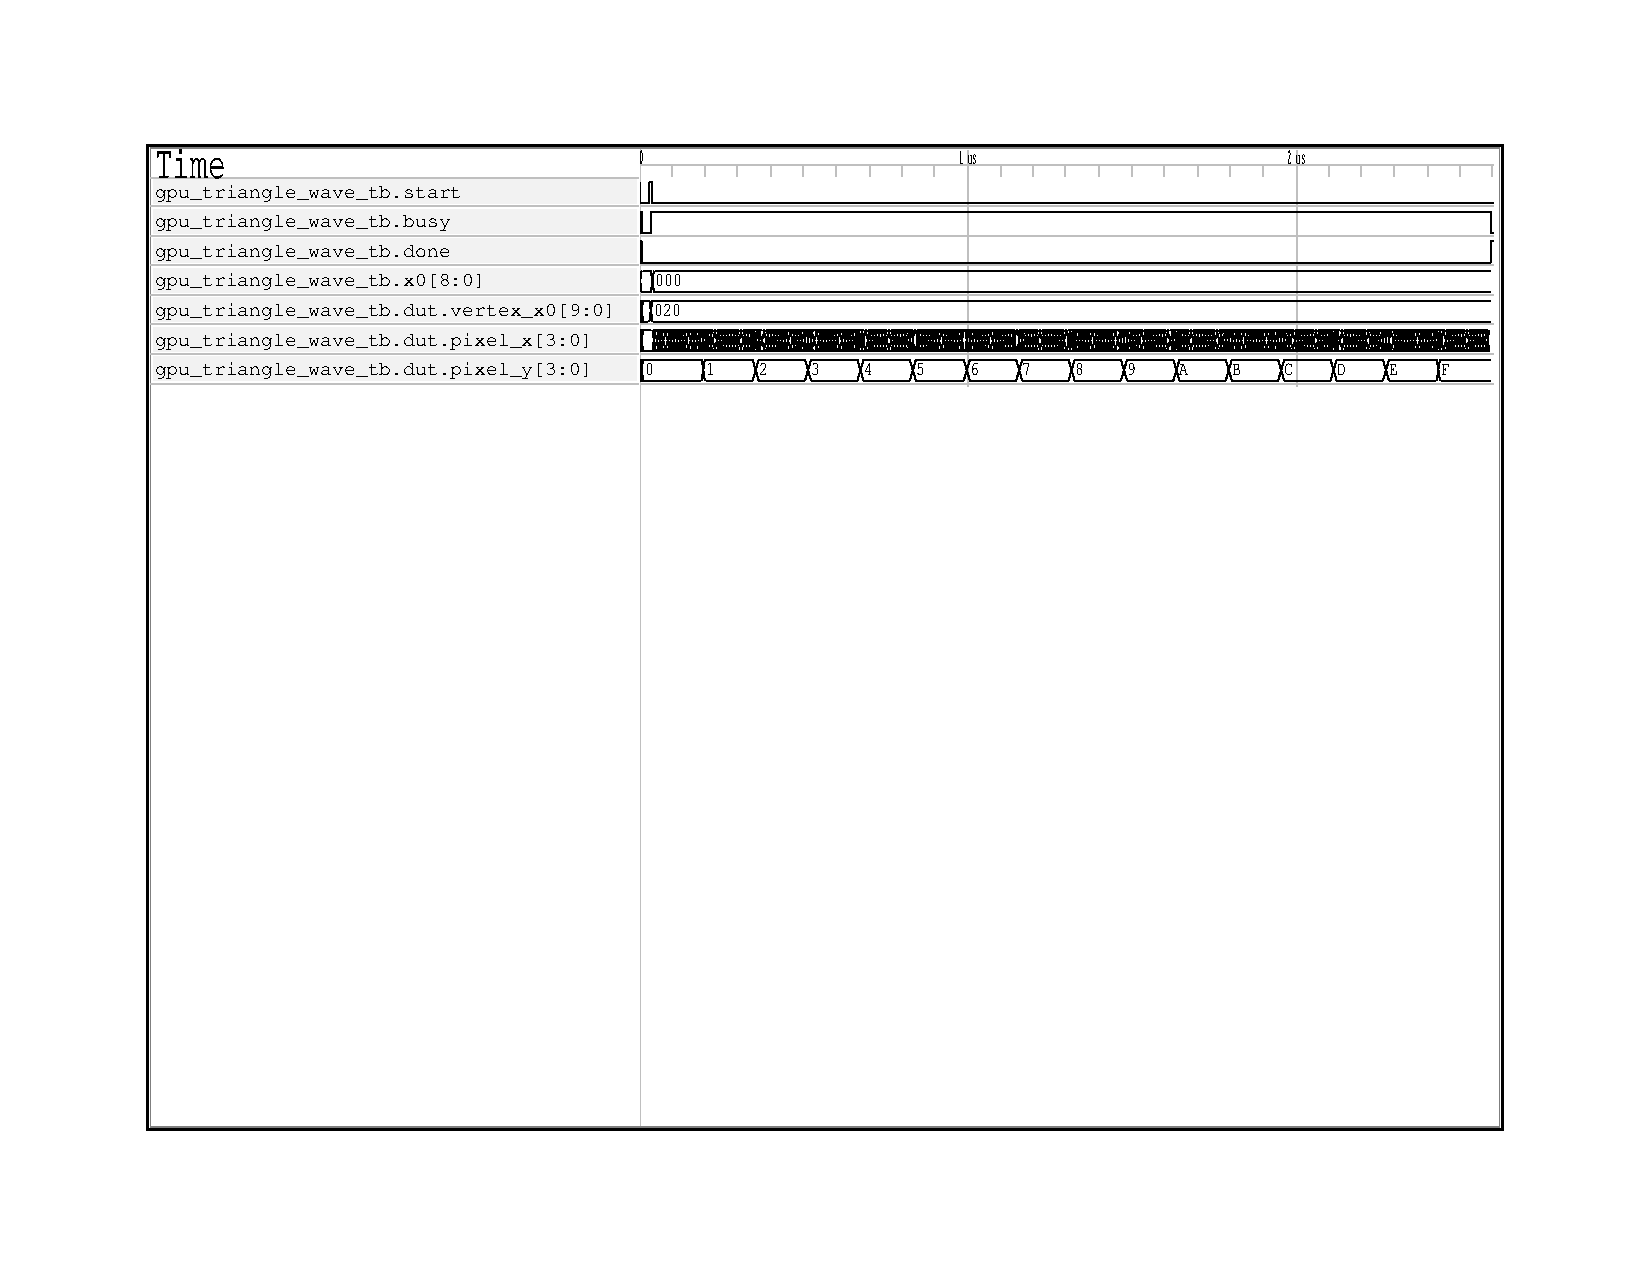
\includegraphics[width=0.92\linewidth,height=0.34\textheight,keepaspectratio]{../data/triangle_wave.pdf}
\caption{Rasterizer RTL trace from the VCD generated by
\texttt{gpu\_triangle\_wave\_tb.sv}. \texttt{busy} spans the scan, \texttt{done}
marks completion, and the external vertex inputs are changed after launch.
The DUT's latched vertex values remain the triangle used for the render.}
\label{fig:rtlwave}
\end{figure}

\section{Matched VLSI measurements}

The three rasterizer arms were implemented for the SkyWater Sky130A process
using the \path{sky130_fd_sc_hd} standard-cell library and OpenLane
v1.0.2 (commit
\texttt{ff5509f65b17bfa4068d5336495ab1718987ff69}; open\_pdks
\texttt{0fe599b2afb6708d281543108caf8310912f54af}). Each run uses the same
35\% target core utilization, 20 ns clock period, library, and physical-flow
configuration; each completes synthesis, placement, clock-tree synthesis,
routing, parasitic extraction, timing analysis, and GDS streaming. The
separate run IDs and source/configuration hashes are recorded in
\texttt{data/physical\_runs.csv}.

\begin{table}[!htbp]
\centering
\scriptsize
\setlength{\tabcolsep}{3pt}
\begin{tabular}{p{0.34\linewidth}p{0.20\linewidth}p{0.20\linewidth}p{0.20\linewidth}}
\toprule
Metric & D: direct & I: incremental & IB: clipped\\
\midrule
OpenLane run & \texttt{21.37.32} & \texttt{23.06.43} & \texttt{23.16.24}\\
Mapped synthesis cells & 7,955 & 8,822 & 9,655\\
Synthesis cell area (\(\mu\mathrm{m}^2\)) & 80,943.88 & 88,885.25 & 91,964.45\\
Final DEF die area (\(\mathrm{mm}^2\)) & 0.24728 & 0.27072 & 0.27981\\
Critical-path metric (\(\mathrm{ns}\)) & 9.57 & 9.93 & 14.07\\
Final \texttt{31-rcx} setup slack (\(\mathrm{ns}\)) & 6.84 & 6.59 & 2.46\\
Final \texttt{31-rcx} hold slack (\(\mathrm{ns}\)) & 0.33 & 0.30 & 0.33\\
MCA setup WNS, min/nom/max (\(\mathrm{ns}\)) & \(-2.21/-2.51/-2.82\) & \(-2.20/-2.34/-2.50\) & \(-10.04/-10.30/-10.56\)\\
Max-fanout violations & 8 & 26 & 18\\
Antenna pin/net violations & \(8/5\) & \(5/5\) & \(11/11\)\\
TritonRoute/Magic DRC violations & \(0/0\) & \(0/0\) & \(0/0\)\\
\bottomrule
\end{tabular}
\caption{Matched OpenLane results for the direct (D), full-frame
incremental (I), and incremental-bounding-box (IB) rasterizers. The
critical-path values are from the flow metrics CSV. The single-corner final
\texttt{31-rcx} slack and the separate min/nom/max-corner (MCA) setup WNS
are shown separately because the reports differ substantially.}
\label{tab:matched-physical}
\end{table}

Relative to D, I increases mapped-cell count by 10.9\% and synthesis area by
9.8\%, while the four tested cycle counts remain unchanged. Its default
\texttt{31-rcx} setup slack is 0.25 ns lower, although its MCA worst setup
WNS is 0.32 ns less negative in the max corner. IB increases mapped-cell
count by 21.4\% and synthesis area by 13.6\%; it offers no scan-cycle
reduction for the full-viewport input, but reduces the reference-triangle
scan from 256 to 121 cycles and the small-triangle scan from 256 to 4.
Its critical-path metric is 47.0\% higher than D's, and its MCA setup WNS
is substantially worse. The results show a workload-dependent trade-off: clipping saves scan cycles
for small triangles, but adds area and worsens the flow's critical-path
metric. They do not establish that recurrence or clipping is inherently
better.

The default final \texttt{31-rcx} reports show positive setup slack, while
the separate MCA reports list negative setup WNS at min, nominal, and max
corners for all three candidates. The nominal-corner result is therefore
not interchangeable with the default single-corner report; this
constraint/corner discrepancy must be reconciled before claiming
all-corner timing closure. The positive single-corner slack is not a
measured silicon clock limit. All runs report zero TritonRoute and Magic
DRC violations, but max-fanout and antenna violations remain. No
\texttt{VSRC\_LOC\_FILES} were supplied, so any IR-drop output is unsuitable
as a calibrated supply-integrity result. No workload-derived power, yield,
or fabricated-silicon evidence is claimed.

\begin{figure}[!htbp]
\centering
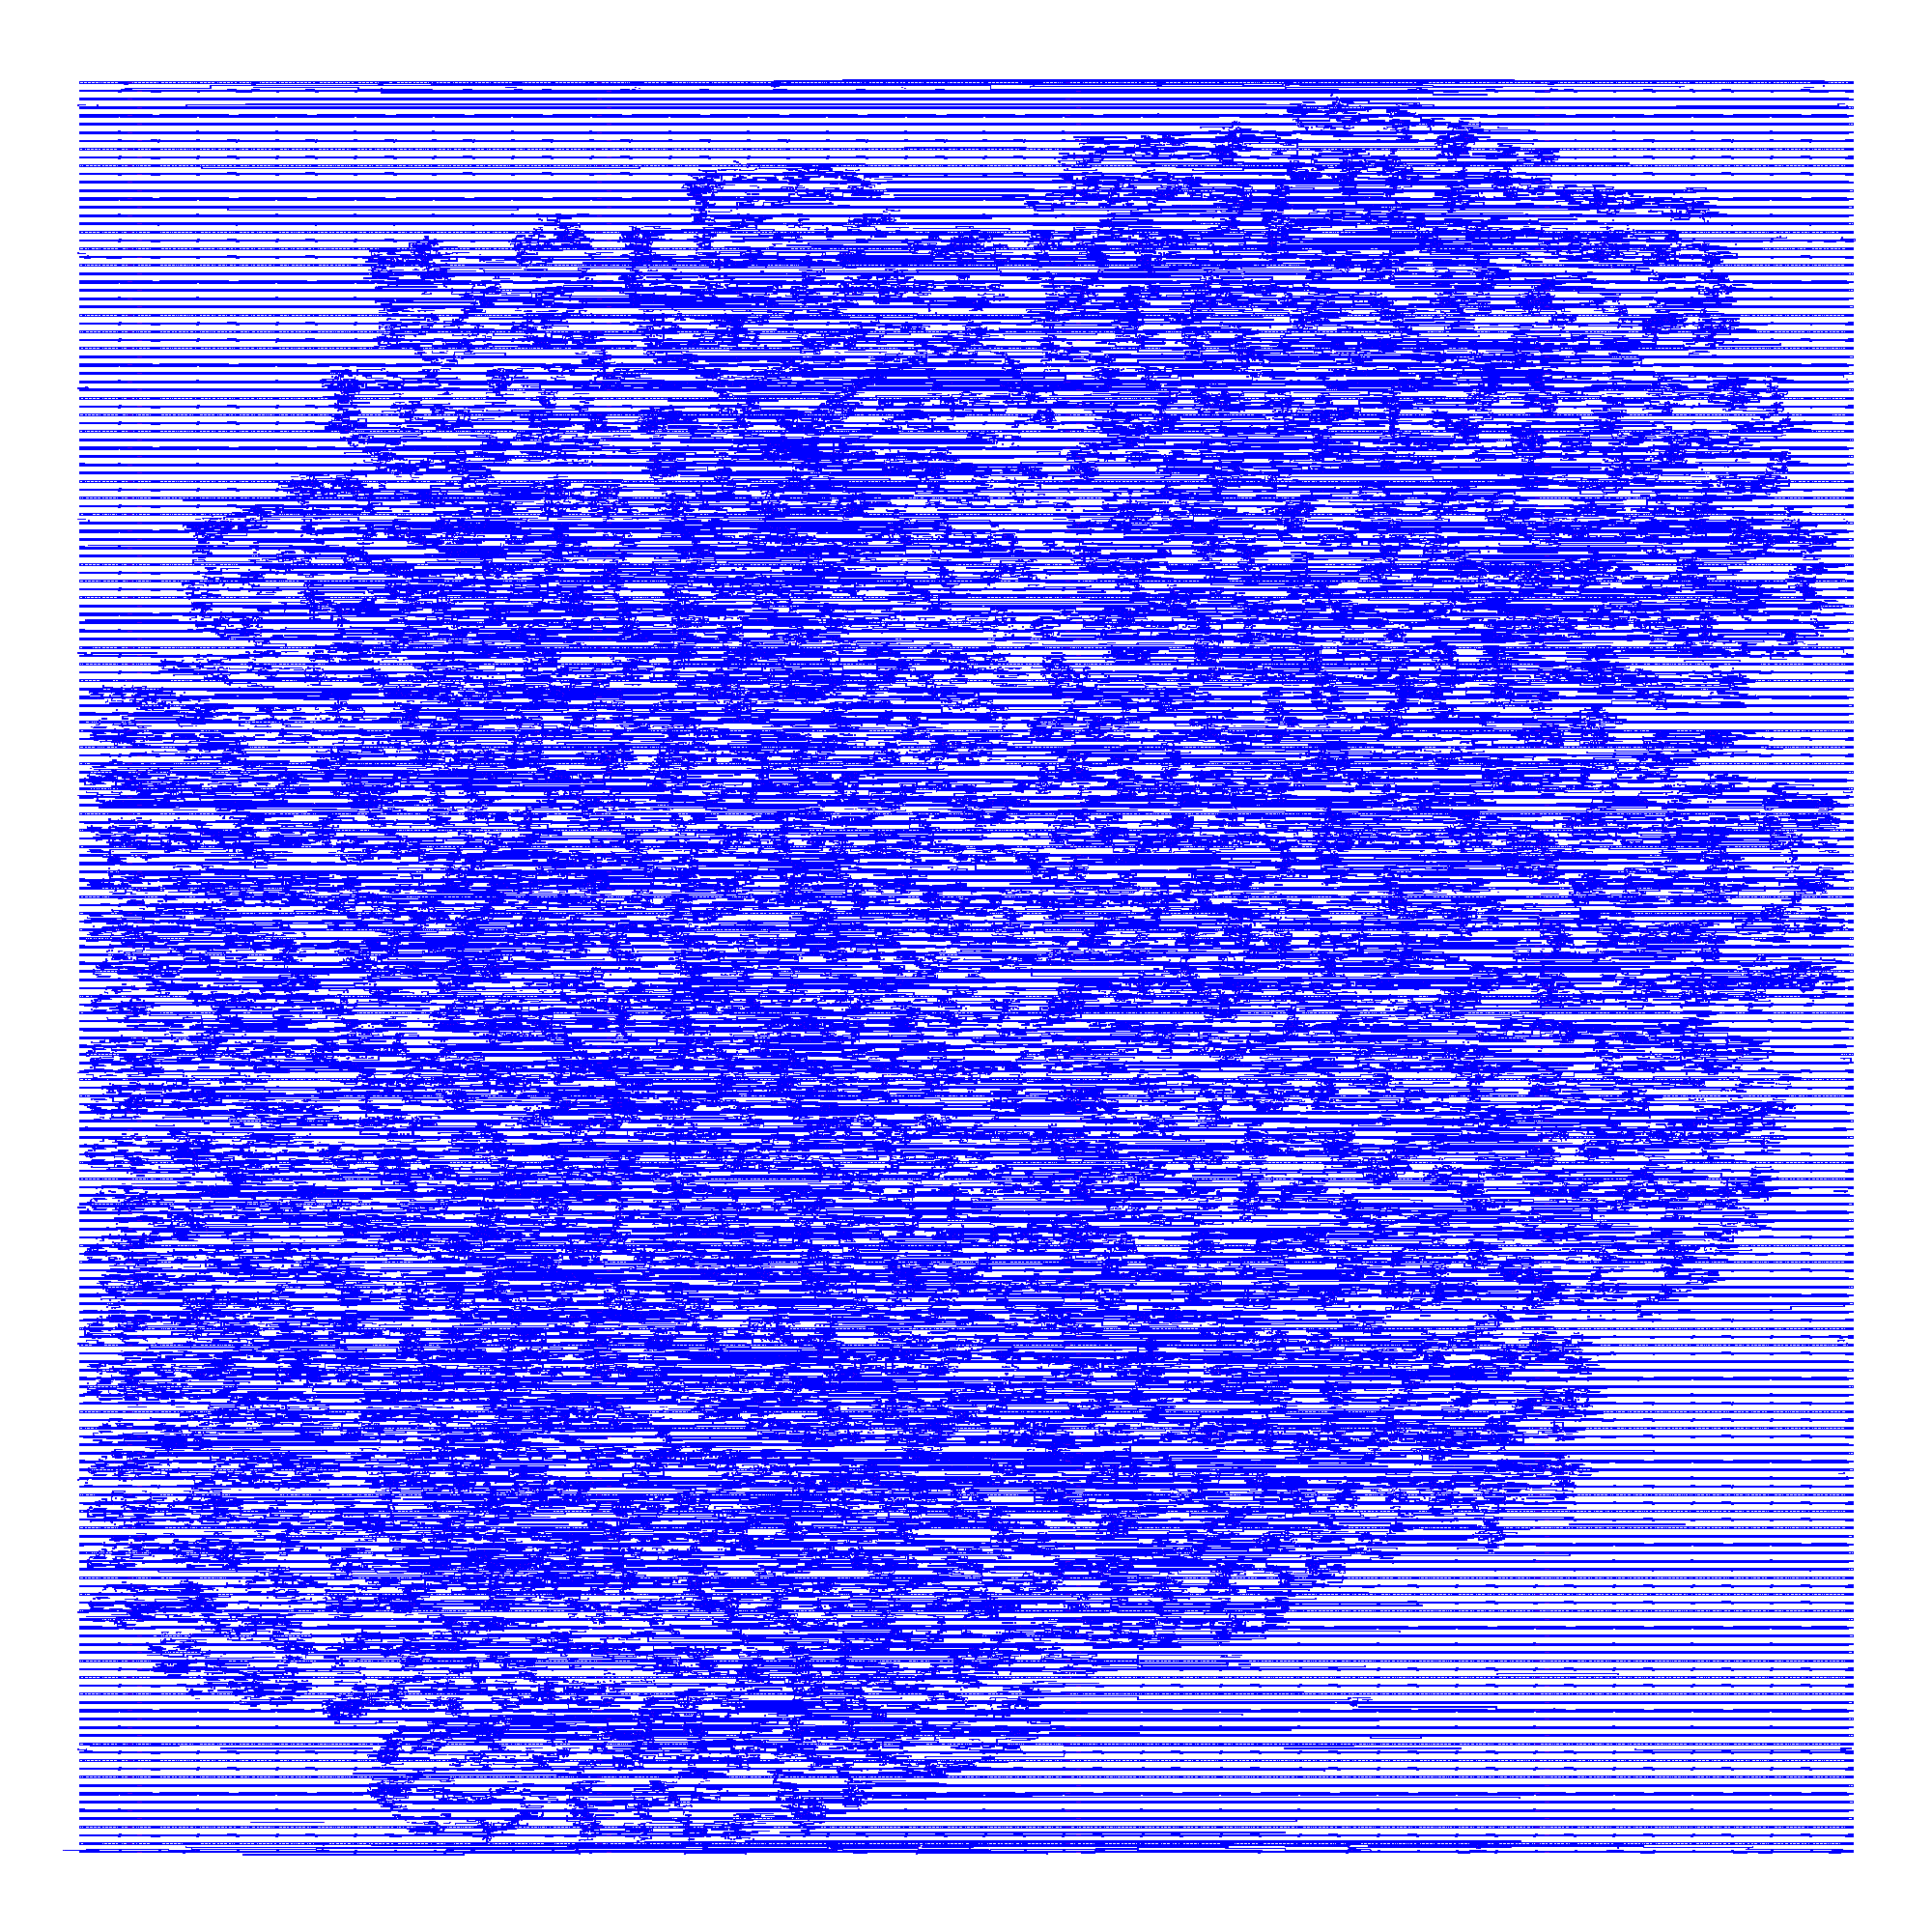
\includegraphics[width=0.55\linewidth,height=0.24\textheight,keepaspectratio]{gpu4x4_floorplan.png}
\caption{KLayout rendering of the saved final GDS for the separate 4-by-4
INT8 matrix engine. The 90-by-90 result in this report is obtained by
repeatedly driving this RTL tile from a simulation testbench; the GDS is not
a physical 90-by-90 matrix array.}
\label{fig:matrix-layout}
\end{figure}

\section{Matched VLSI design-space experiment}

\subsection{Matched architecture arms}

The controlled factor is the edge-evaluation/traversal microarchitecture.
All candidates must preserve the same ports, one-bit framebuffer, start-time
input snapshot, signed coordinate encoding, pixel-center samples, inclusive
edge rule, and exact 20-bit signed arithmetic contract.

\begin{table}[!htbp]
\centering
\small
\begin{tabular}{p{0.12\linewidth}p{0.36\linewidth}p{0.40\linewidth}}
\toprule
Arm & Datapath and traversal & Status\\
\midrule
D & Current direct edge-function evaluation at each of 256 viewport
samples. & Implemented, functionally checked, and physically measured.\\
I & Initialize the three edge values once, then update them with constant
per-pixel increments; scan all 256 samples. & Implemented, functionally
checked, and physically measured.\\
IB & Use the same incremental edge recurrence, but scan only the clipped,
conservative bounding box of pixel centers. & Implemented, functionally
checked, and physically measured.\\
\bottomrule
\end{tabular}
\caption{Implemented RTL comparison arms. D versus I isolates the recurrent
edge datapath; I versus IB isolates the effect of bounded traversal. D has
the smallest mapped area and shortest critical-path metric in the measured
runs; IB has lower cycle counts for the two smaller test cases.}
\label{tab:arms}
\end{table}

For an edge \(a\rightarrow b\), the edge value changes by
\[
E(x+1,y)=E(x,y)-16(b_y-a_y),\qquad
E(x,y+1)=E(x,y)+16(b_x-a_x),
\]
because adjacent pixel centers are 16 fixed-point units apart. These
increments are exact integers; no approximation is introduced by the
recurrence. For IB, the candidate scan bounds are derived from the condition
that a pixel center lies between the minimum and maximum vertex coordinate:
\[
x_{\min}=\max\!\left(0,\left\lceil
\frac{\min_i x_i-8}{16}\right\rceil\right),\quad
x_{\max}=\min\!\left(15,\left\lfloor
\frac{\max_i x_i-8}{16}\right\rfloor\right),
\]
with analogous expressions for \(y\). Empty clipped bounds complete with
zero pixel evaluations. The box is conservative: it may test uncovered
pixels but must not exclude any covered pixel. The signed floor/ceiling
operations must be implemented explicitly; relying on language-specific
integer division for negative coordinates is disallowed.

The per-edge update count gives a transparent operation model. Let \(w\)
and \(h\) be the number of pixel centers in the clipped box and \(P=wh\).
Direct evaluation performs six multiplications and three product subtractions
per sample edge triplet, for approximately \(6P\) products and \(3P\)
subtractions, in addition to the signed coverage tests. I instead performs
three initial edge evaluations, then three edge additions for each
horizontal or vertical recurrence step:
\[
N_{\mathrm{add},I}=3\big((w-1)h+(h-1)\big),\qquad
N_{\mathrm{add},IB}=3\big((w-1)h+(h-1)\big).
\]
For I, \(w=W,h=H\); for IB, \(w,h\) are the clipped box dimensions. The
recurrence replaces repeated products with stored edge state and additions;
it does not eliminate per-sample sign comparisons or coverage writes. This
operation model predicts work, not standard-cell area, delay, or power.

For the tested 16-by-16 viewport, the direct/I sample count is \(WH=256\).
The reference triangle has a conservative 11-by-11 box (\(P=121\)); the
small triangle has a 2-by-2 box (\(P=4\)). The observed cycle model is
\[
C_D=C_I=256,\qquad C_{IB}=P
\]
for nondegenerate cases with a nonempty clipped box. Degenerate inputs
complete without a scan in all three variants. A nondegenerate triangle
outside the viewport still incurs 256 scan cycles in D and I, whereas IB
detects its empty clipped box and completes without pixel evaluations.
These equations describe this RTL schedule, not silicon throughput.

\subsection{Research questions and observed results}

\begin{enumerate}[leftmargin=2em]
  \item \textbf{RQ1 --- logic mapping:} at equal semantics and target
        constraints, how do synthesis area and mapped cell composition
        change from repeated edge evaluation to edge accumulators? In this
        implementation, I instead maps to more cells and area; the RTL
        operation-count reduction alone did not predict mapped cost.
  \item \textbf{RQ2 --- timing and physical effects:} which paths limit
        setup after placement and routing, and do the arithmetic recurrences
        reduce the worst path or merely move it to initialization/control?
        Compare extracted slack, critical-path start/endpoints, path cell
        classes, fanout, buffering, and routed violations.
  \item \textbf{RQ3 --- latency versus area:} how does bbox occupancy
        interact with IB's initialization/control cost? Measure actual
        completion cycles per workload; do not infer performance from a
        single full-screen triangle.
  \item \textbf{RQ4 --- Pareto quality:} which candidates are nondominated
        in synthesis area, final die area, extracted timing, and workload
        latency? There is no single winner unless a target area or latency
        constraint is specified in advance.
  \item \textbf{RQ5 --- power:} how do workload-dependent switching activity
        and energy per completed triangle differ among the matched candidates?
        Power is in scope, but current reports provide only vectorless
        estimates; workload-derived power and energy remain unmeasured.
\end{enumerate}

The physical runs test these hypotheses in one open-PDK flow. The observed
area increase for I shows that reducing repeated edge evaluation in the
algorithm does not guarantee a smaller synthesized circuit: recurrence
state, initialization, muxing, and control also map to cells. The IB
results quantify the cost of occupancy-aware traversal in this implementation:
the reference and small inputs save 135 and 252 scan cycles, respectively,
but the added bound arithmetic increases the critical-path metric from
9.57 ns (D) to 14.07 ns (IB), and its max-corner setup WNS is \(-10.56\) ns.
For this 16-by-16 case, D has the smallest mapped area and shortest
critical-path metric. IB reduces scan cycles on sparse inputs, but its
critical-path metric and max-corner setup WNS are worse. These results apply
to the tested RTL, constraints, tools, and workloads. Pineda's edge-function
formulation is prior art \cite{Pineda1988}; this experiment measures how
equivalent recurrence and traversal choices map into an open standard-cell
flow.

\subsection{Controls, workloads, and measurements}

All arms use the same RTL parameter widths, port semantics, reset behavior,
framebuffer capacity, Sky130 HD library, PDK revision, OpenLane/OpenROAD
versions, clock and I/O constraints, utilization target, synthesis strategy,
and physical-design settings. Each candidate has a clean, separately
identified run; run IDs, source/configuration hashes, and the common flow
settings are recorded in \texttt{data/physical\_runs.csv}. The saved run
directories preserve the netlists, final DEF/GDS, SPEF, and signoff reports.

The 136-triangle suite is useful for regression, but does not represent a
production workload. A larger performance study should publish a
fixed-seed corpus stratified by clipped-box occupancy, including
off-screen, small, medium, near-full-frame, near-degenerate,
boundary-touching, and both-winding cases. For every input, compare the
complete framebuffer against the same wide-integer reference and check
busy/done behavior, reset, starts while busy, and input changes after
launch.

Report synthesis cell area/count, final die/core area, extracted timing,
corner-specific WNS, routing warnings, DRC violations, and RTL cycles for
each arm. The final OpenLane reports also include the typical-corner
vectorless estimates in Table~\ref{tab:power-estimates}. They have no
workload VCD/SAIF annotation and cannot establish workload power or energy.
A useful comparison needs aligned activity traces for the same
occupancy-stratified inputs, with library, voltage, corner, parasitics, and
active/idle window held constant. Report internal, switching, and leakage
power separately, then integrate over each render to calculate energy per
triangle. Do not infer this from gate counts, RTL operation counts, or the
inverter ngspice test.

These single-run physical results do not sample
placement-seed variability. Future workload studies should report
min/median/p95/max cycles by occupancy class and a Pareto frontier over
absolute area, timing, and per-workload latency; avoid a composite score
without a predeclared design objective.

\begin{figure}[!htbp]
\centering
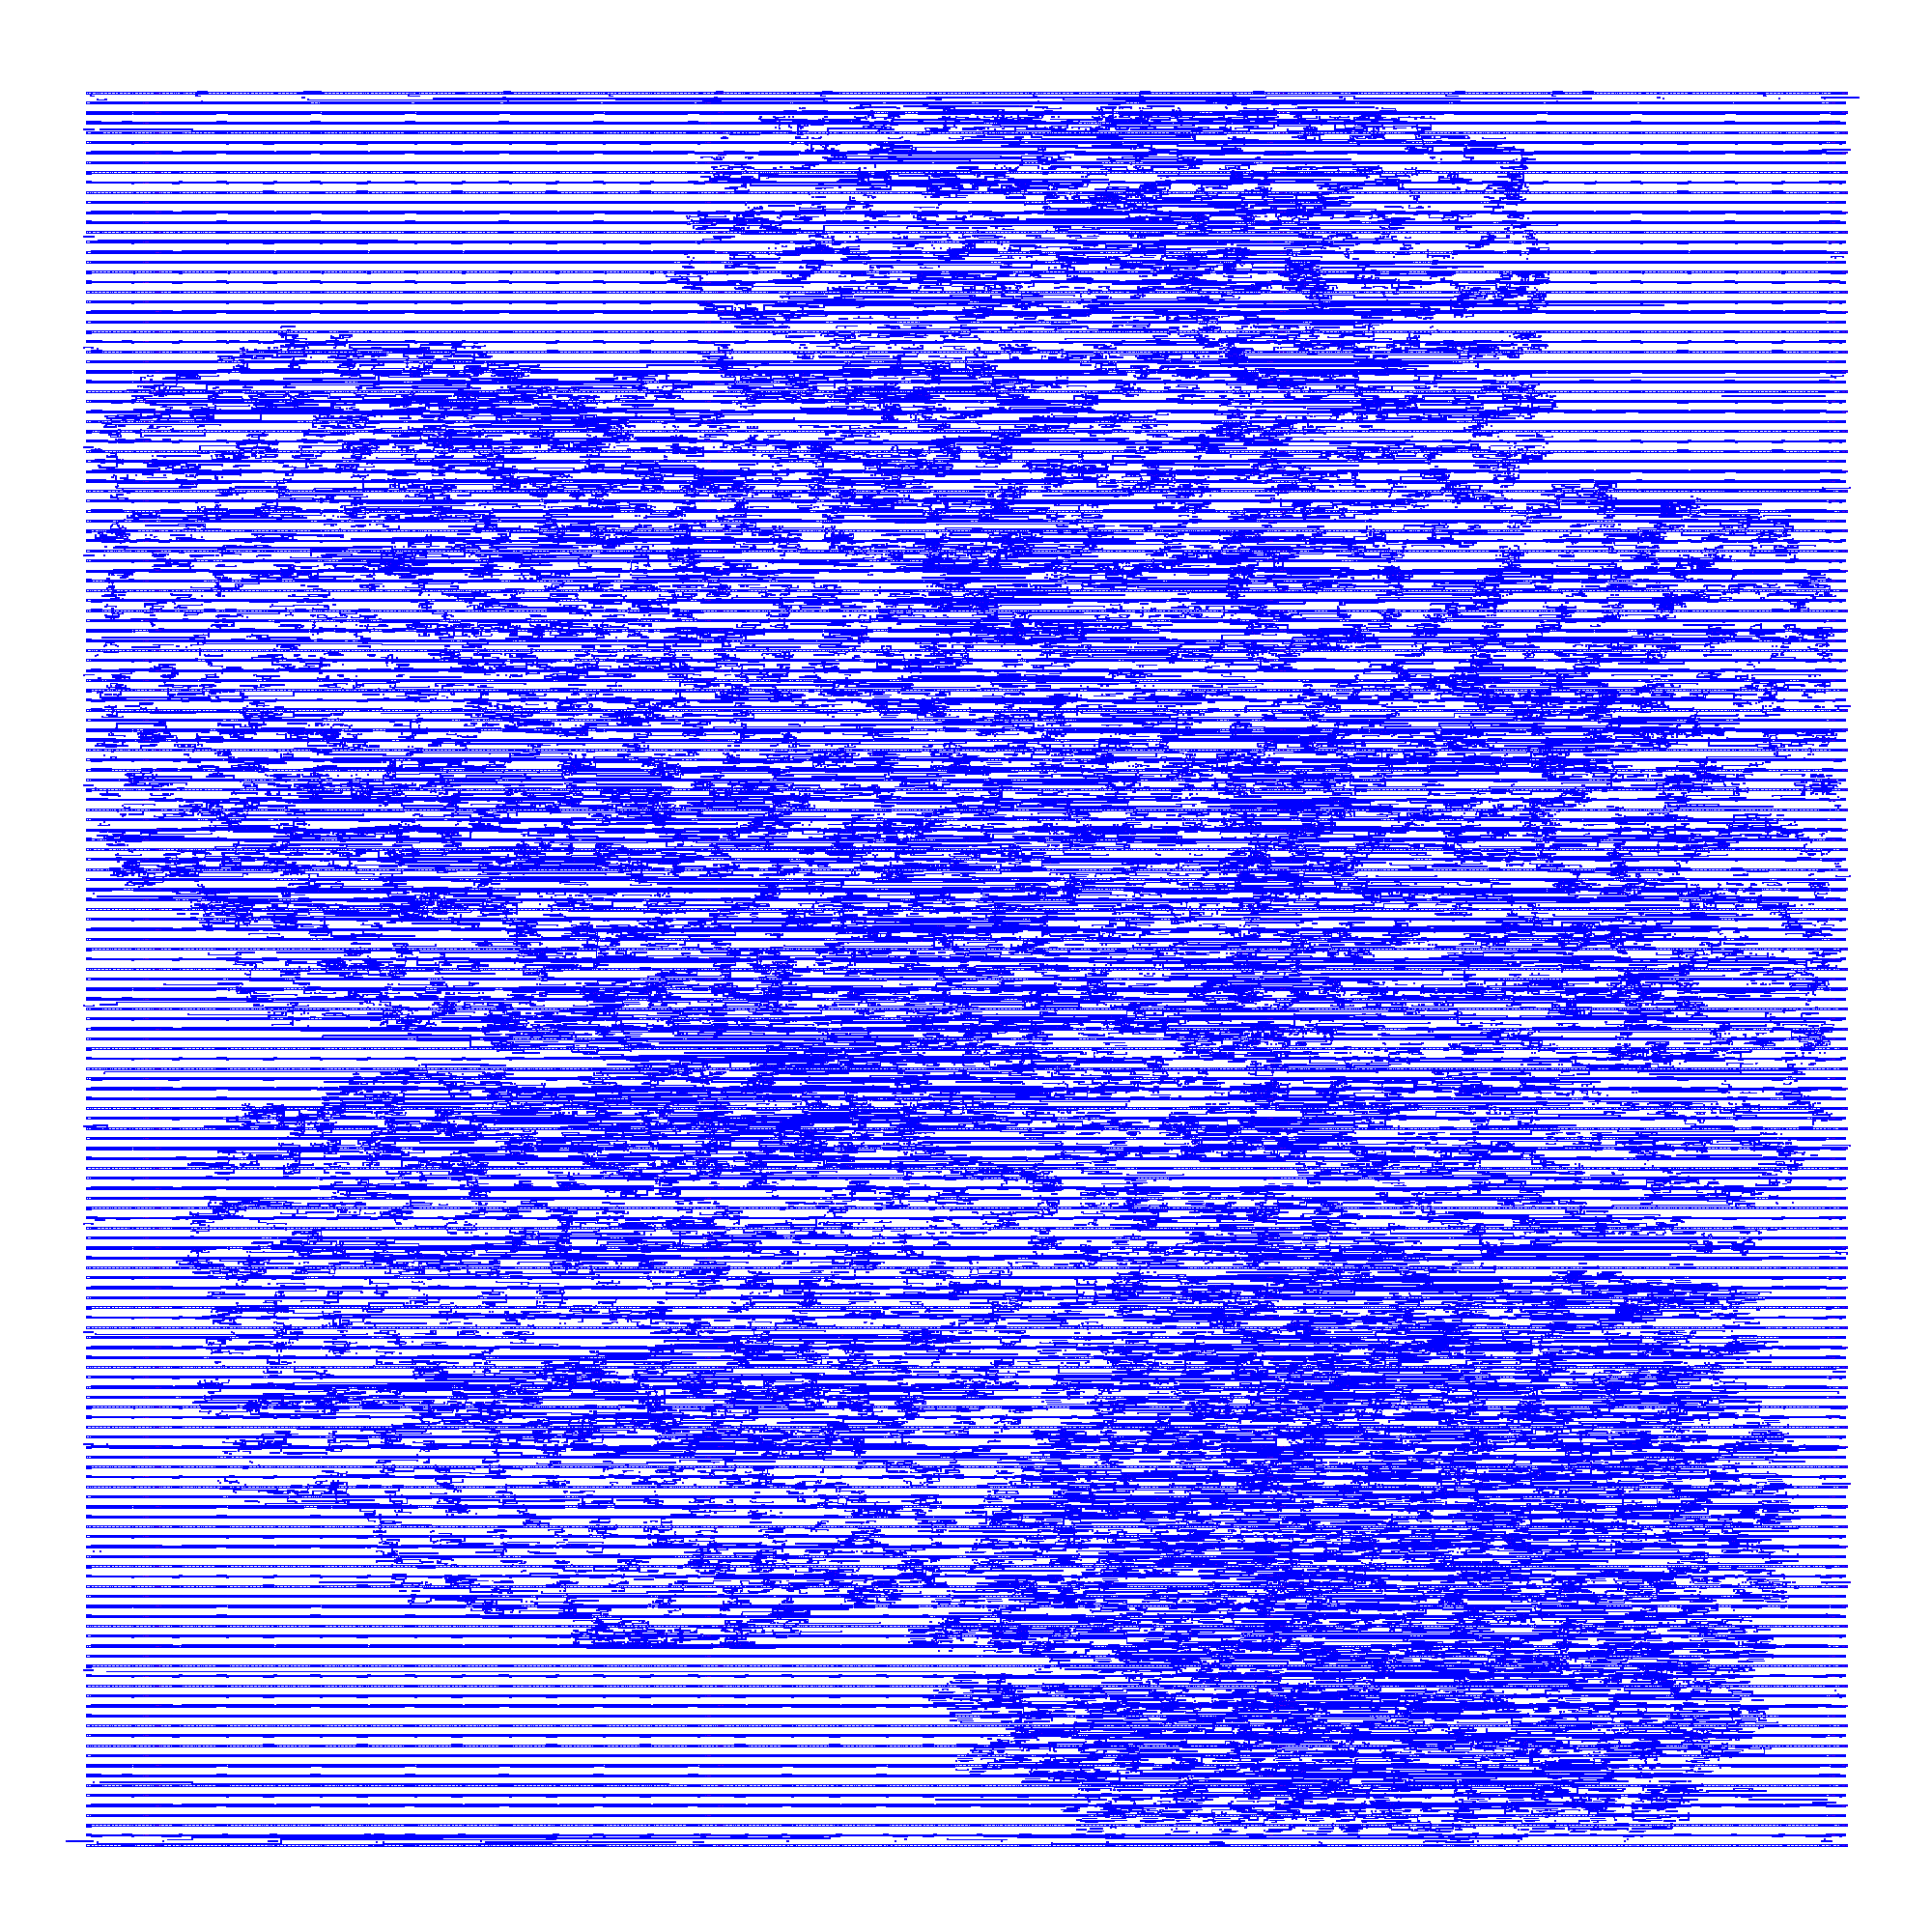
\includegraphics[width=0.32\linewidth]{gpu_triangle_floorplan.png}
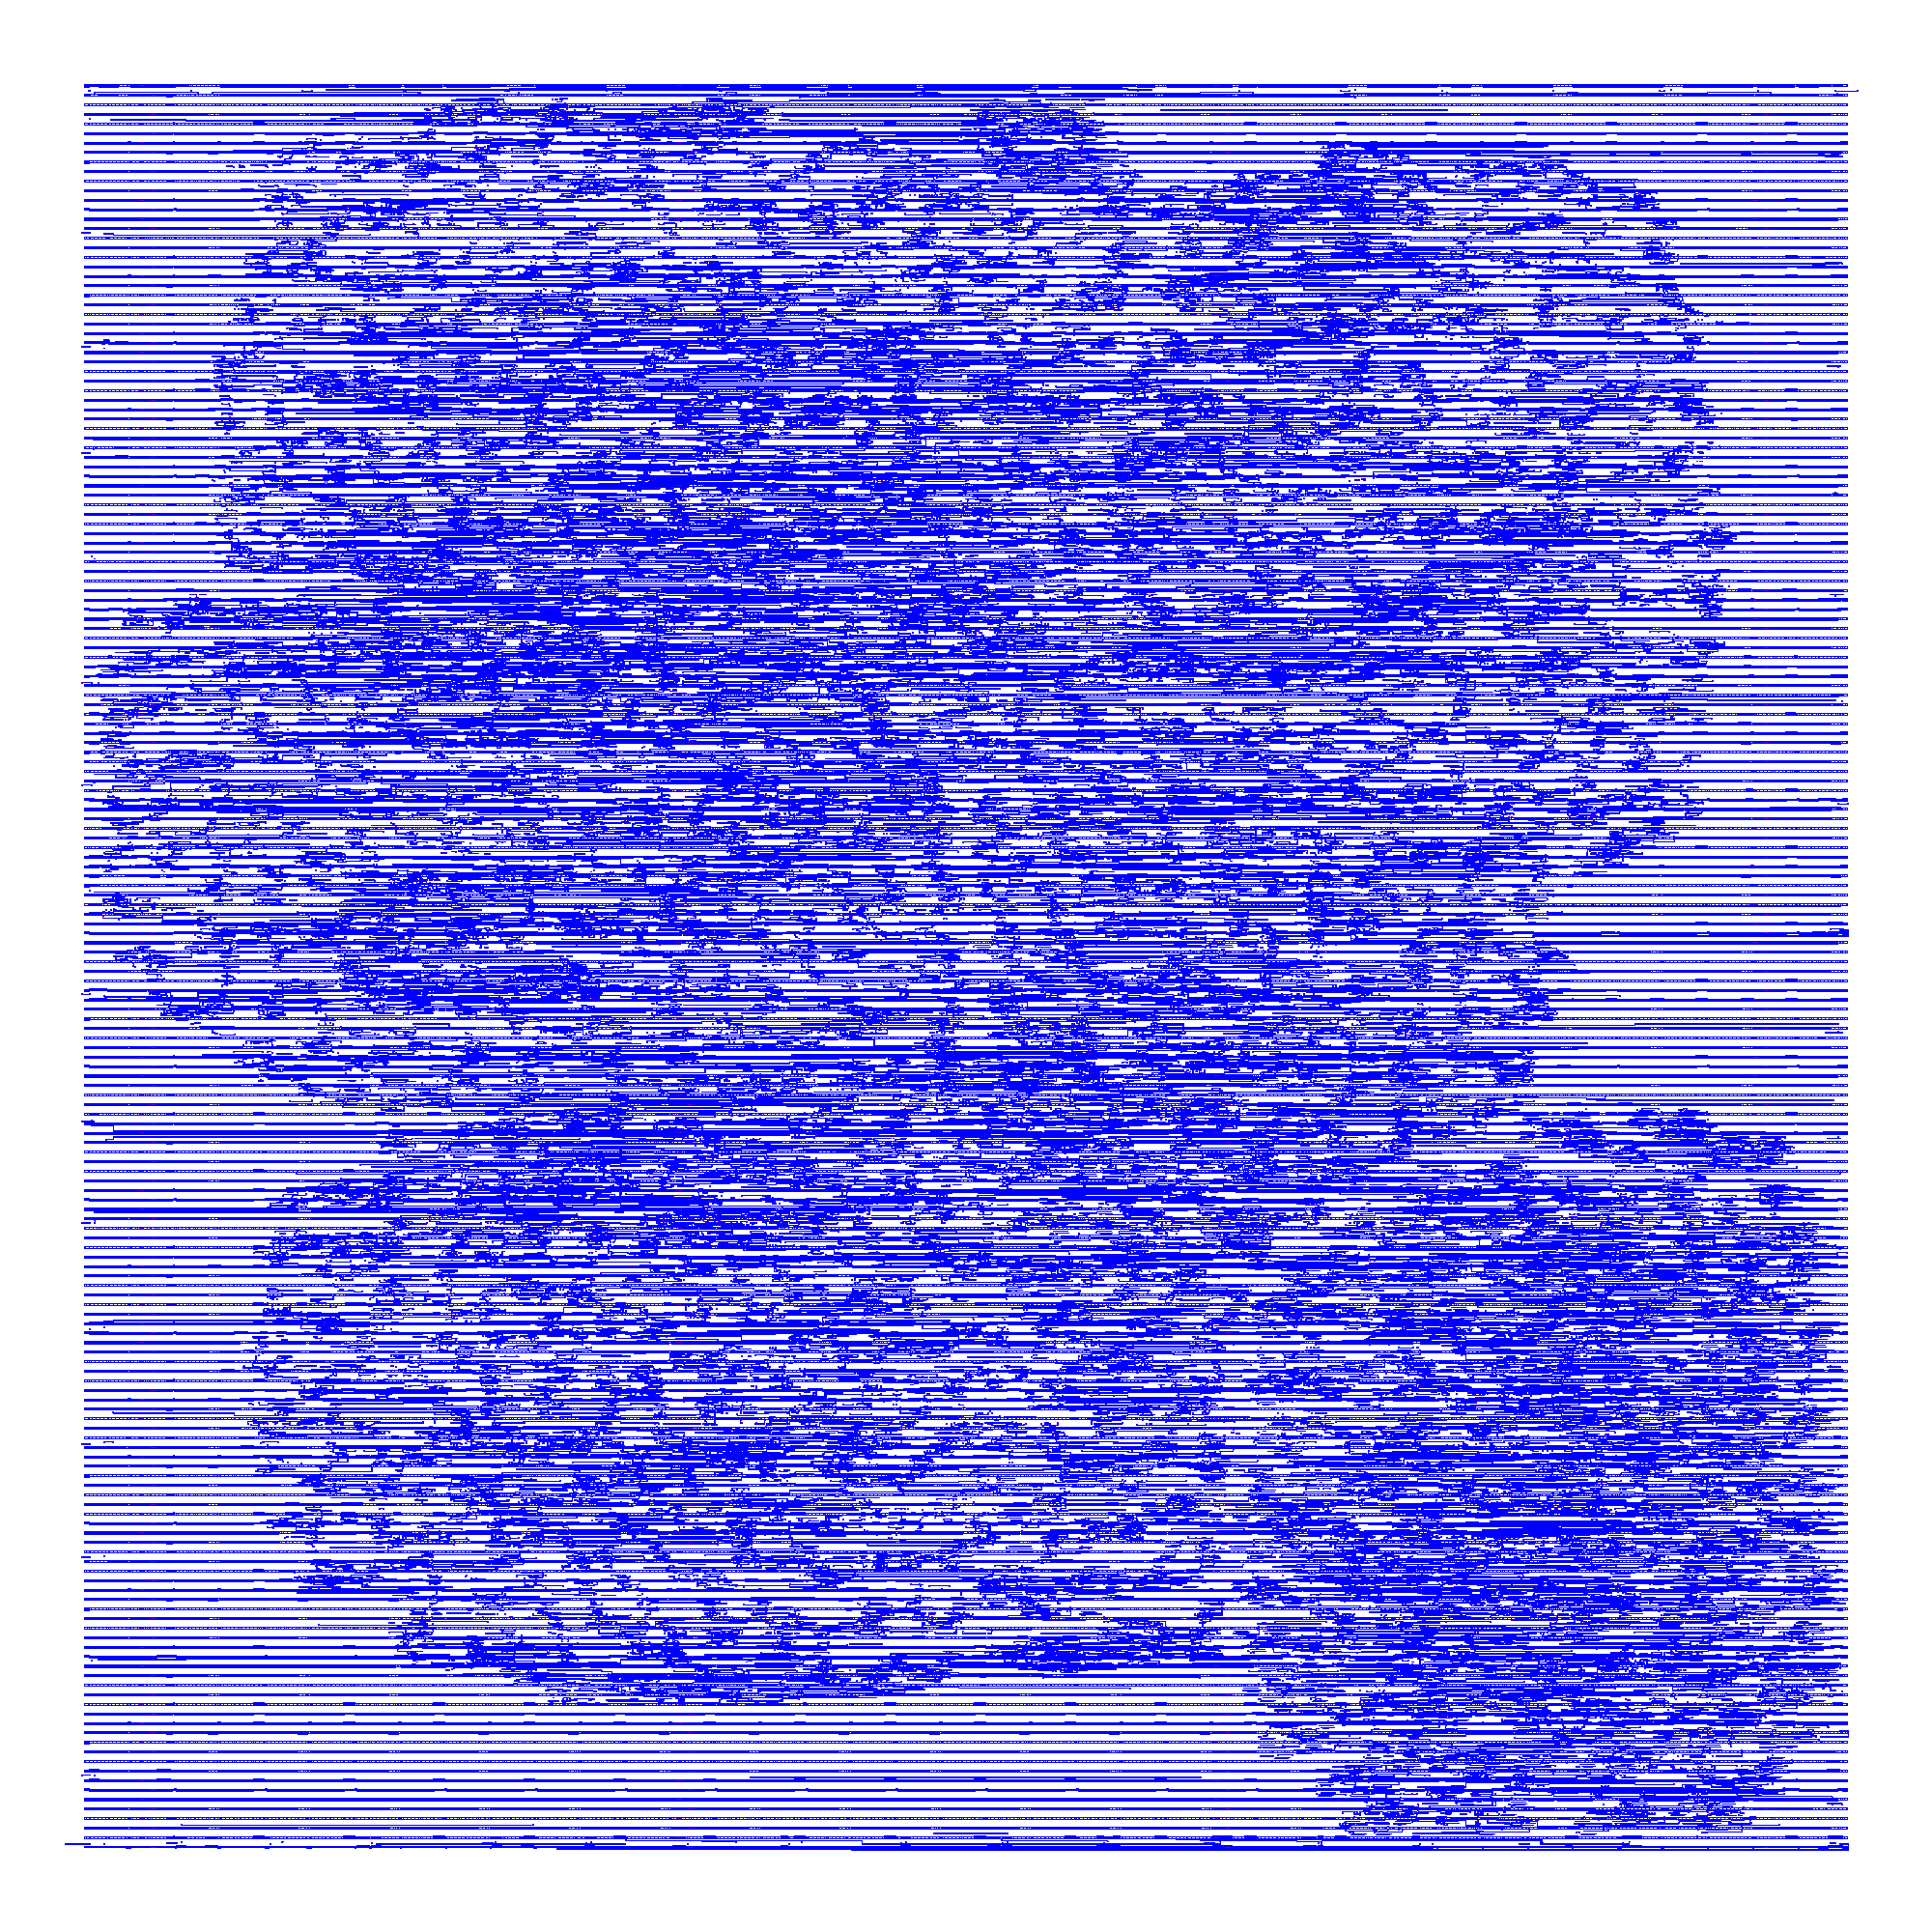
\includegraphics[width=0.32\linewidth]{gpu_triangle_incremental_floorplan.png}
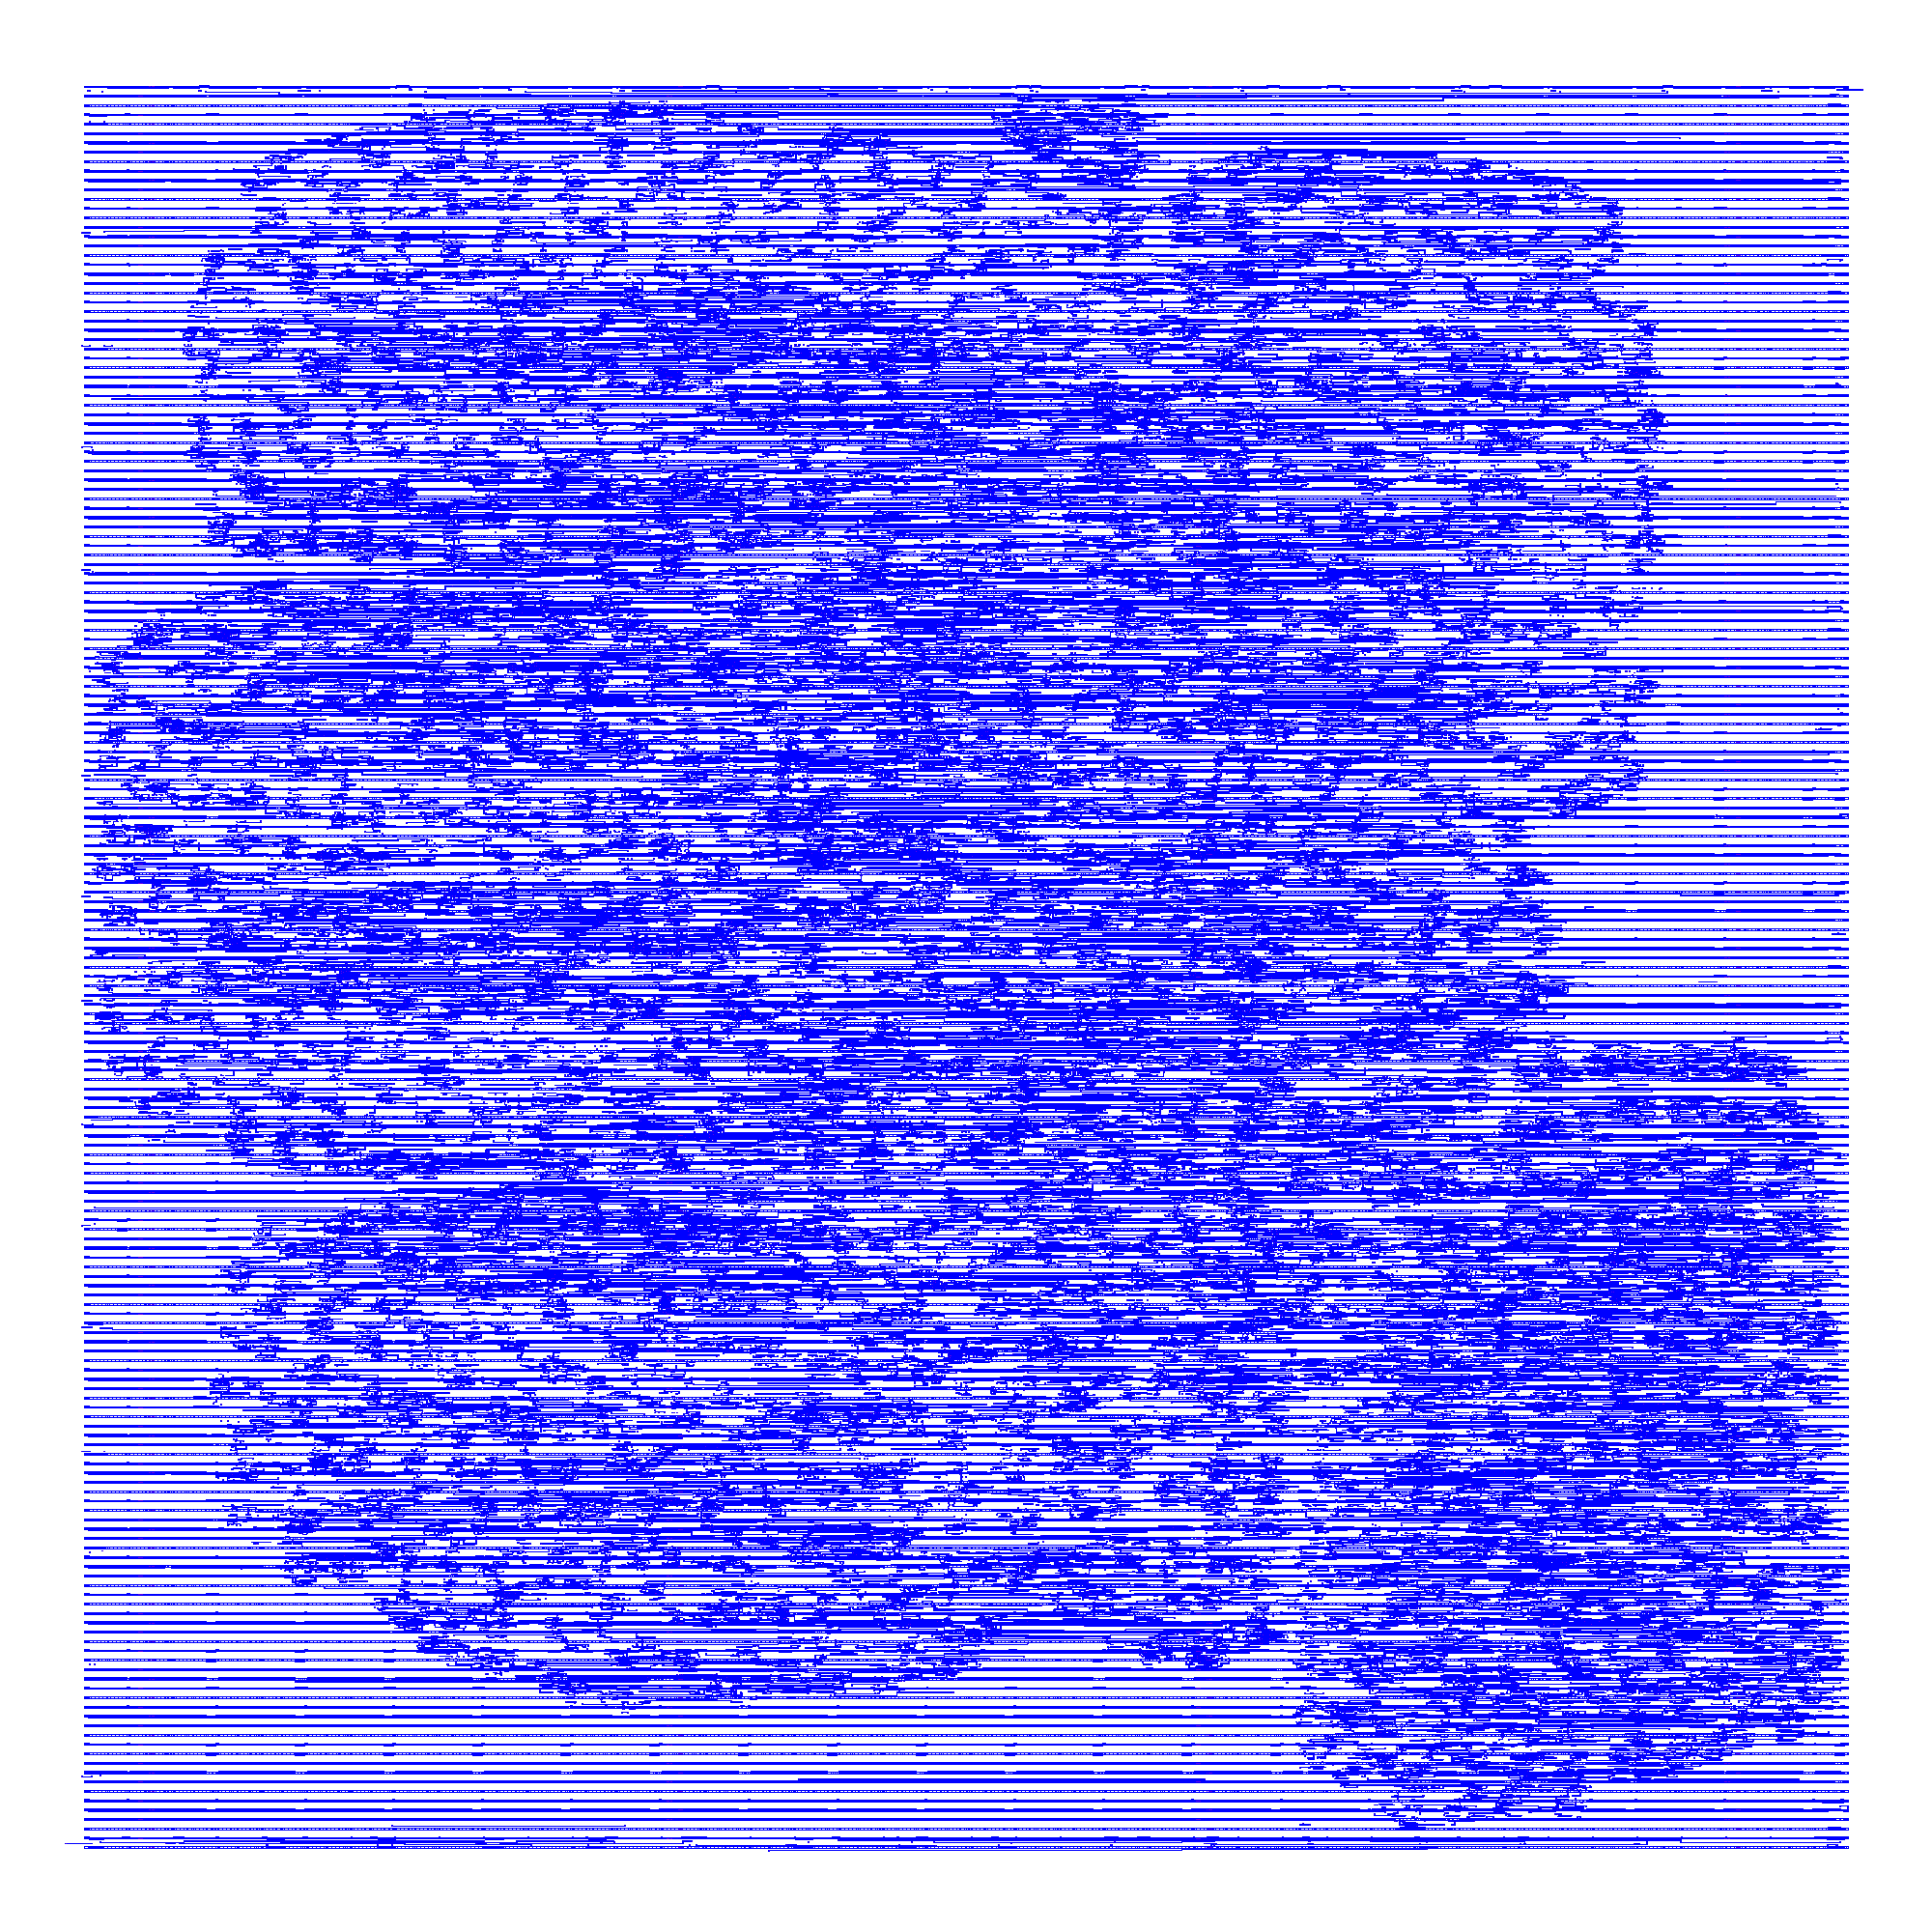
\includegraphics[width=0.32\linewidth]{gpu_triangle_incremental_bbox_floorplan.png}
\caption{KLayout renders of the saved final routed GDS for D (left), I
(center), and IB (right). These are physical-design artifacts, not
floorplans annotated with functional regions; each panel is fitted
independently and should not be used to compare dimensions visually.}
\label{fig:baseline-layout}
\end{figure}

\begin{figure}[!htbp]
\centering
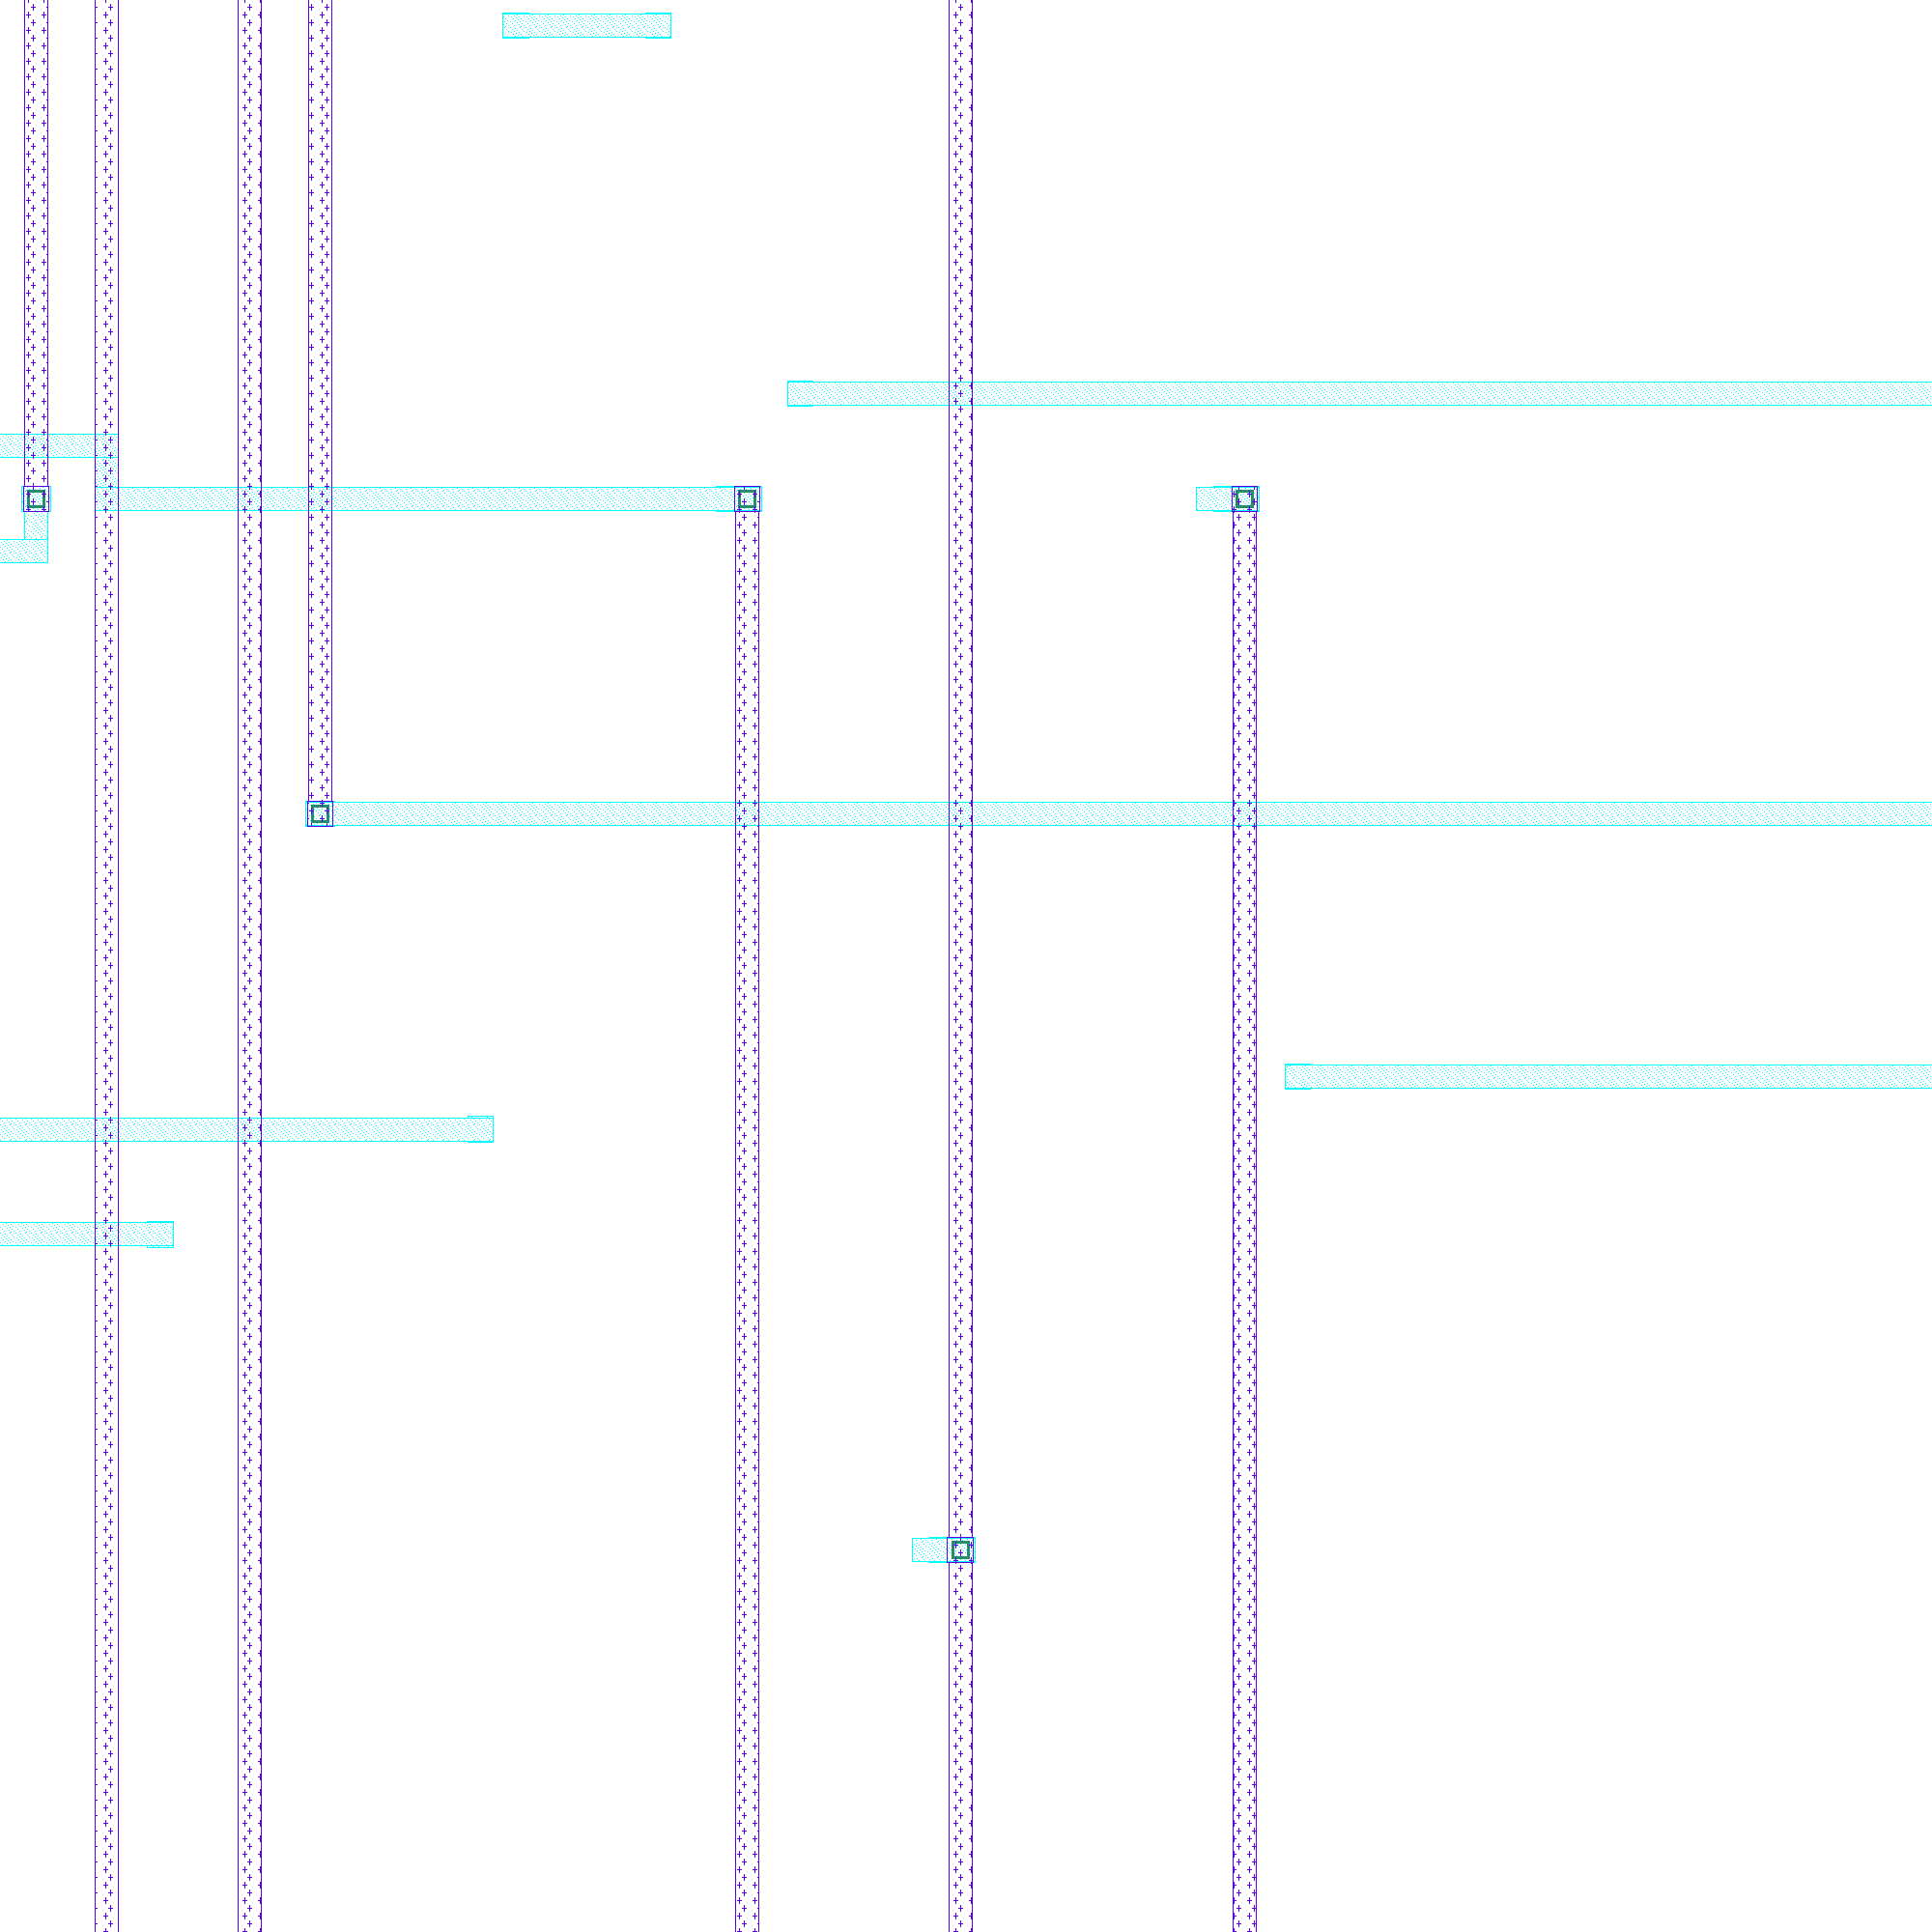
\includegraphics[width=0.82\linewidth]{gpu_triangle_layout_detail.png}
\caption{A KLayout render of a \(25\,\mu\mathrm{m}\times25\,\mu\mathrm{m}\)
window from the rasterizer's final routed GDS. The view isolates selected
upper routing layers and suppresses text labels. The colored lines are
physical routing geometry; they are not a functional block diagram. The
matching final GDS is the authoritative layout artifact.}
\label{fig:layout}
\end{figure}

\subsection{Preliminary power estimates}

The saved final \texttt{31-rcx} OpenLane/OpenSTA reports include a
typical-corner \texttt{report\_power} result for each rasterizer. No
workload-derived VCD or SAIF activity was annotated, so these are vectorless
estimates under OpenSTA's default activity assumptions. They are flow
outputs, not workload measurements, and are not used to rank the variants.
The ngspice test simulates one inverter, not either accelerator.
These estimates cover only the rasterizer. No workload power or energy was
measured for the matrix tile. A separate matrix study should report energy
per useful MAC or per completed 90-by-90 multiplication.

\begin{table}[!htbp]
\centering
\small
\begin{tabular}{lrrrr}
\toprule
Arm & Internal (mW) & Switching (mW) & Leakage (nW) & Total (mW)\\
\midrule
D & 15.10 & 18.70 & 52.6 & 33.80\\
I & 8.43 & 9.84 & 57.2 & 18.27\\
IB & 11.00 & 13.50 & 58.2 & 24.50\\
\bottomrule
\end{tabular}
\caption{Typical-corner vectorless power estimates copied from the matched
OpenLane runs' final STA reports. Rounded component totals may differ from
the unrounded totals; the machine-readable source is
\texttt{data/power\_estimates.csv}. These are not activity-annotated workload
measurements.}
\label{tab:power-estimates}
\end{table}

\section{Limitations and threats to validity}

\begin{itemize}[leftmargin=1.5em]
  \item \textbf{Workload coverage:} D, I, and IB have passed the same
        136-case RTL reference suite and four-case cycle benchmark, but four
        fixed performance inputs do not represent a production scene or
        establish a workload-wide speedup.
  \item \textbf{Verification:} the 136-case deterministic test suite and
        four benchmark inputs are limited; they are not exhaustive or formal
        proofs. A fixed-seed, stratified corpus and protocol assertions are
        required for the proposed comparison.
  \item \textbf{Power:} the reported typical-corner values are vectorless
        OpenSTA estimates, not workload-annotated power or energy.
        Default activity assumptions may not represent the relative
        switching of D, I, and IB. No candidate has activity-annotated
        accelerator energy; the standalone inverter ngspice experiment is
        not a substitute.
  \item \textbf{Design representation:} the GPU kernels are described in
        RTL and were not captured as Xschem transistor-level schematics.
        The separate ngspice inverter test does not validate the accelerator
        datapaths or their power.
  \item \textbf{Physical signoff:} max-fanout and antenna warnings remain.
        Default single-corner summaries show positive setup slack, but the
        explicit min/nom/max MCA reports show negative setup WNS for every
        arm; this discrepancy must be resolved. The default VSRC placement
        limits IR-drop interpretation. No fabricated silicon or measured
        accelerator power is available.
  \item \textbf{Generalization:} a 16-by-16, one-bit framebuffer in Sky130 HD
        is a deliberately small case study. Results will not directly
        generalize to larger resolutions, other libraries, or full GPU
        pipelines.
\end{itemize}

\section{Reproducibility}

The reproduction script reruns the RTL regressions and benchmarks, exports
the GTKWave trace, renders the saved GDS files with KLayout, extracts the
saved OpenLane power estimates, and builds the PDF. It requires Icarus
Verilog, GTKWave, KLayout, Python 3, Ghostscript's \texttt{ps2pdf}, and
LaTeX/BibTeX. From the repository root, run:
\begin{verbatim}
./designs/gpu4x4/research_report/tools/reproduce.sh
\end{verbatim}
The script reads the saved OpenLane runs; it does not rerun the physical
flow. The matrix test uses the 4-by-4 RTL tile in Icarus and does not create
a 90-by-90 layout. To rerun the physical designs, use OpenLane v1.0.2, the
recorded Sky130A PDK revision, and the saved configurations. Raw traces,
simulation logs, and the PPM output are kept in the data directory. The
power summary is vectorless; the script does not generate activity traces.

\section{Conclusion}

The project has verified two separate RTL workloads: 16-by-16 triangle
coverage and a testbench-driven 90-by-90 INT8 matrix product using a 4-by-4
tile. The three rasterizers pass the shared reference suite and have matched
Sky130 RTL-to-GDS runs. Incremental stepping did not reduce scan cycles or
area in these runs; bounding-box traversal shortened the two smaller
benchmark cases while increasing area and the critical-path metric. The
multi-corner reports do not show timing closure, and workload energy has not
been measured. Next, resolve the timing-corner discrepancy, expand the
published workload corpus, and collect comparable activity traces before
making power or energy claims.

\bibliographystyle{plain}
\bibliography{references}
\end{document}
